\documentclass[conference]{IEEEtran}

% wenn ein Fehler kommt zu Incompatible package cite, dass Paket auskommentieren
\usepackage{cite}
\usepackage{amsmath,amssymb,amsfonts}
\usepackage{verbatim} % um viele zeilen auszukommentieren
\usepackage{algorithmic}
\usepackage{listings}
\usepackage{siunitx}
\lstset{
	language=Python,
	basicstyle=\ttfamily\small,
	aboveskip={1.0\baselineskip},
	belowskip={1.0\baselineskip},
	columns=fixed,
	extendedchars=true,
	breaklines=true,
	tabsize=4,
	frame=lines,
	showtabs=false,
	showspaces=false,
	showstringspaces=false,
	keywordstyle=\color[rgb]{0.627,0.126,0.941},
	commentstyle=\color[rgb]{0.133,0.545,0.133},
	stringstyle=\color[rgb]{01,0,0},
	numbers=left,
	numberstyle=\small,
	stepnumber=1,
	numbersep=10pt,
	captionpos=t,
	escapeinside={\%*}{*)}
}


% Zur Verwendung von Hyperlinks im Dokument. PDF ist anklickbar.
% https://latex.org/forum/viewtopic.php?t=25067
\usepackage{hyperref}
\hypersetup{colorlinks=true, pdfstartview=FitV, linkcolor=blue, citecolor=black, plainpages=false, pdfpagelabels=true, urlcolor=blue}
\usepackage[all]{hypcap}

\usepackage[svgpath=/img/]{svg}


\usepackage{graphicx}
%--------------------------------
\usepackage[ngerman]{babel}
\usepackage[utf8]{inputenc}
\usepackage[T1]{fontenc}
\usepackage[backend=biber,defernumbers=false]{biblatex}
% Wenn Quellen über filecontents im Dokument eingefügt werden
%\addbibresource{bib.bib}

\bibliography{Literatur}
%\usepackage[ngerman]{babel}		% Achtung umlaut 
%\usepackage[utf8]{inputenc}       % UTF-8 ist wichtig,  ASCII hat nicht alle Schriftzeichen  
%-----------------------------------
\usepackage{textcomp}
\usepackage{xcolor}
\usepackage{dirtytalk} % nein, nicht was du denkst.  Packet hilft  gegen verschluckte gänsefüschen
\def\BibTeX{{\rm B\kern-.05em{\sc i\kern-.025em b}\kern-.08em T
		\kern-.1667em\lower.7ex\hbox{E}\kern-.125emX}}
\usepackage{minted}
\setminted{breaklines,breakanywhere}

%---------------------------
\defbibfilter{wissenschaftlich}{%
	not type=online and not type=thesis
}
\defbibfilter{nichtWissenschaftlich}{%
	type=online or type=thesis
}

\begin{document}
	
	
	
	\title{rosBerry - ein autonomer Roboter auf Basis von ROS und eines Modellautos mit Maker-Elektronik}
	
	\author{\IEEEauthorblockN{1\textsuperscript{st} Welter, Heike}
		\IEEEauthorblockA{ 
			Heike.Welter@stud.hs-mannheim.de}%
		\and
		\IEEEauthorblockN{2\textsuperscript{nd} Matheis, Steffen}
		\IEEEauthorblockA{
			Steffen.Matheis@stud.hs-mannheim.de }
		\and
		\IEEEauthorblockN{3\textsuperscript{rd} Barsalou, Marie }
		\IEEEauthorblockA{ 
			Marie.Barsalou@stud.hs-mannheim.de}
	}
	
	\maketitle
	
	\begin{abstract}
		Ziel von Projekt rosBerry besteht darin, einen kleinen, schnellen aber dennoch preisgünstigen Roboter aus leicht verfügbaren Standardbauteilen zu bauen.
		Zusätzlich soll er mit dem Robot Operating System betrieben und mit einer Künstlichen Intelligenz versehen werden.
		Der Roboter soll einen optischen Marker erkennen und darauf zufahren.
		Frontalzusammenstöße mit Wänden soll er dabei vermeiden.
	\end{abstract}
	\begin{comment}
	Tipp zur Verbesserung:
	Ein Abstract sollte folgende 4 Fragen sehr kompakt beantworten:
	1. Worum geht es allgemein?
	2. Welches Problem wird hier konkret betrachtet?/gelöst?
	3. Worin besteht die wesentliche Lösung?
	4. Was ist das wesentliche Ergebnis?
	Das ist schwer zu schreiben, aber aus Sicht eines Lesers sehr informativ. 
	\end{comment}
	
	\begin{IEEEkeywords}
		Roboter, ROS, Raspi, Neuronale Netze, Arduino
	\end{IEEEkeywords}
	
	%\section{Einleitung }  wollen wir  eine machen?
	%projekteinleitung text hier
	\section{Theorie zu Roboter und seiner Künstlichen Intelligenz}
	
	
	Wenige Projekte in Robotik oder Künstlichen Intelligenz für Autonome 
	Systeme existieren, ohne das es nicht andere vergleichbare Projekte gibt. 
	Eine vollständige oder zumindest Repräsentative Darstellung würde den 
	Rahmen einer Studentischen Projektarbeit sprengen.
	
	\subsection{Vergleichbare Hardwareansätze — Donkey Cars} %mary
	%Donkey car infos
	Die Hardware des Roboters wurde vom Donkey Car Projekt inspiriert.
	Das Donkey Car Projekt beschäftigt sich damit, ein ferngesteuertes Auto mit einem Raspberry Pi zu steuern.
	Mehr Informationen zu diesem Projekt gibt es auf ihrer Website https://docs.donkeycar.com.
	Donkey Cars fahren größtenteils mit Hilfe von quelloffenem Python Code. \\
	\\
	Auf Youtube hat ein Benutzer namens Tiziano Fiorenzani gezeigt, wie ein Donkey Car mit ROS betrieben werden kann.
	Das Video https://youtu.be/iLiI\_IRedhI verweist auf Github für Tiziano 
	Fiorenzanis Code. Es wurde eine Abzweigung eines Github-Repositoriums 
	erstellt. Auf 
	\url{https://github.com/Wifi-cable/Robotic_AI_student_project/}
	%\href{https://github.com/Wifi-cable/Robotic_AI_student_project/}{Quellcode
	% }
	Findet sich der Quellcode des Projektes. 
	Das Projekt wurde um einen Arduino und mehrere ROS Knoten sowie um 
	Launchfiles erweitert.
	
	
	\subsection{Vergleichbare Projekte zur Künstlichen Intelligenz} %steffen ? mary?
	Das Neuronale Netz zur Bildklassifizierung ist an das Buch \glqq Artificial Intelligence for Robotics\grqq  \cite{govers2018artificial} angelehnt.
	Darin vermittelt F. Grovers, wie Künstliche Intelligenz für Autonome Systeme funktionieren kann, indem er zeigt, wie er einem kleinen Roboter beibringen würde aufzuräumen.
	In einem Kapitel beschreibt der Autor, dass der Roboter mit Hilfe von Neuronalen Netzen lernen soll, ob sich Spielzeuge auf dem Teppich befinden, um sie später aufzuräumen.\\
	
	Auch die Bachelorarbeit \glqq Bildklassifikation auf einem Raspberry Pi Zero am Beispiel einer Ladestationserkennung \grqq \cite{Amanda} von Amanda Decker ist ein vergleichbares Projekt.
	Einige der Grundansätze aus dieser Arbeit wurden für dieses Projekt übernommen.
	So haben wir das Neuronale Netz nicht auf einem Raspberry Pi trainiert und einen Marker genommen der sich gut rotieren und spiegeln lässt.
	Somit kann jedes Bild des Datensatzes gespiegelt werden, um mit mehr Daten arbeiten zu können.
	%Anders als Amanda Decker jedoch haben wir uns für Keras entschieden, statt eine selbstgeschriebene Künstliche Intelligenz zu verwenden.
	
	\section{Theoretische Grundlagen von Projekt rosBerry}
	In diesem Kapitel wird auf die Erstellung des Datensatzes für die KI eingegangen sowie auf die Grobübersicht des Softwaresystems auf die Knotenarchitektur. %Wuhuuu Einführungssatz (Kann sich nochmals ändern.)
	
	\subsection{Ansätze für die Erstellung des Datensatzes}	%mary
	\begin{figure} %[!h]
		\centering
		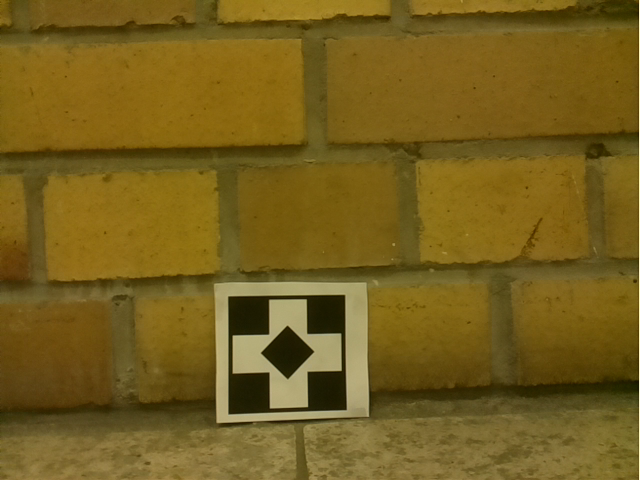
\includegraphics[width=9cm]{img/data1455211246.png}
		\caption{Der Optische Marker den die KI suchen wird }
		\label{Marker}
	\end{figure}
	
	Bei Amanda Deckers Bachelorarbeit schien die KI Schwierigkeiten damit zu haben, zwischen dem Marker und einem Blauton zu unterscheiden, der auch im Marker vorkam.
	Es schien auch schwierig zu sein ein Binärbild vom Marker zu erzeugen, da die beiden Farben des Markers einen geringen Kontrast zueinander haben.
	Da Kameras in Opencv mit Hilfe von Schachbrettmustern kalibriert werden, wird für dieses Projekt ein Symbol mit ähnlich hohem Kontrast und scharfen Kanten verwendet.
	\\
	
	Dieses Symbol\ref{Marker} ist nicht nur in 4 Richtungen rotierbar, sondern auch zweifach spiegelbar, ohne den Marker zu verfälschen. (Rotationsinvarianz und Spiegelungsinvarianz)
	Es verfügt auch über einen maximalen Kontrast und klare, gerade Kanten.
	\\
	\noindent
	Ein Neuronales Netz kann nur so gut sein wie die Daten, mit denen es trainiert und getestet wurde.
	In vielen wissenschaftlichen und populärwissenschaftlichen Artikeln wurde beschrieben, wie ein ungeeigneter Datensatz zu unbrauchbaren Ergebnissen führte.
	So wurden Vorurteile der Forscher bestätigt, oder die KI traf Entscheidungen anhand von falschen Kriterien, wie der Bildunterschrift statt des Bildinhalts.
	\\
	Um einen möglichst robusten Datensatz zu bekommen, werden verschiedene Techniken angewendet:
	\begin{itemize}
		\item Um zu verhindern, dass die KI alle Bilder mit starken Kontrasten für einen Marker hält, wird ein Ausschnitt einmal mit und einmal ohne den Marker fotografiert.
		\item Gegen den \glqq schön-wetter KI\grqq-Effekt (eine KI die annimmt jedes gut ausgeleuchtete Bild muss ein Treffer sein) wird der Marker bei verschiedenen Beleuchtungen fotografiert.
		Dazu gehören direktes Sonnenlicht, Schatten, künstliche Beleuchtung mit LED, Lampen und Neonröhren. 
		\item Um zu verhindern, dass die KI alles für ihren Marker hält, was eine gewisse Größe hat und quadratisch ist, wurde der Marker aus verschiedenen Distanzen fotografiert. 
		\item Gegen Noise-Anfälligkeit wurden verschiedene Hintergründe bei den Fotos verwendet. Teils weiße Wände, teils strukturierte Hintergründe oder eine Freifläche. 
		\item Um zu verhindern, dass sich die KI auf die Bildmitte konzentrieren kann, wird der Marker aus verschieden Positionen fotografiert. 
	\end{itemize}
	
	
	\subsection{Grobübersicht über das System}
	In diesem Kapitel werden wir, bevor wir näher auf die Softwarearchitektur und den Hardwareaufbau von rosBerry eingehen, das System kurz als Gesamtüberblick vorstellen.
	
	\begin{figure}%[!ht]
		\centering
		%\includesvg[width=9cm]{Gesamtsystem.svg}
		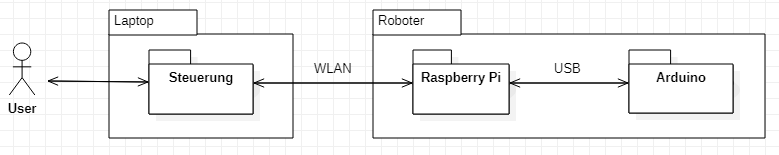
\includegraphics[width=9cm]{img/Gesamtsystem.PNG}
		\caption{Gesamtüberblick des Systems}
		\label{Gesamtzusammenhang}
	\end{figure}
	Die Abbildung \ref{Gesamtzusammenhang} zeigt das System, welches auf mehreren Komponenten basiert.
	Innerhalb des Systems wird eine Software eingesetzt, die auf dem Robot Operating System (ROS) basiert.
	Diese Software läuft verteilt auf den Komponenten Laptop, Raspberry PI und Arduino, wie in Abbildung \ref{Gesamtzusammenhang} zu sehen.
	\\
	Beginnen werden wir mit der Komponente Laptop.
	Sie ist dazu da, dem User die Steuerung des Roboters zu ermöglichen.
	Die Steuerung kann erst erfolgen, wenn auf dem Raspberry Pi ein Accesspoint geöffnet wurde, mit dem sich der Laptop — der Nutzer letztendlich — via WLAN verbindet.
	\\
	Innerhalb der anderen Komponente Roboter — unser rosBerry — befindet sich die beiden Hardware-Elemente Raspberry Pi und ein Arduino. Roscore läuft auf dem Raspberry PI und ein Node - für den Ultraschallsensor - auf dem Arduino.
	
	Der Arduino wird durch ein USB Kabel mit dem Raspberry Pi verbunden.
	Dadurch wird eine Kommunikation ermöglicht, in welcher der Arduino den Raspberry Pi in Zeitabständen mit Sensordaten versorgt.
	\\
	An dieser Stelle ist anzumerken, dass weitere Hardware verwendet wird, die im Kapitel Hardwareaufbau näher vorgestellt wird.
	
	%----------------------------------------------------------------
	\subsection{Architektur der ROS-Knoten}\label{sec:Architektur}
	
	%heike
	%grobstruktur,  nodes topics und all das was es schon als text gibt
	In diesem Kapitel wird die Software-Architektur des Roboters vorgestellt.
	%Den dazugehörige Quellcode finden Sie auf https://github.com/Wifi-cable/Robotic\_AI\_student\_project.
	%An dieser Stelle möchten wir darauf hinweisen, dass das Repository von Tiziano Fiorenzani geklont wurde.
	%Die Dokumentation seines Projektes finden Sie unter folgende Verlinkung zu Youtube https://youtu.be/iLiI\_IredhI.
	
	% Das Bild später bei Existenz aller Knoten aktualisieren.
	\begin{figure}[!ht] 
		\centering
		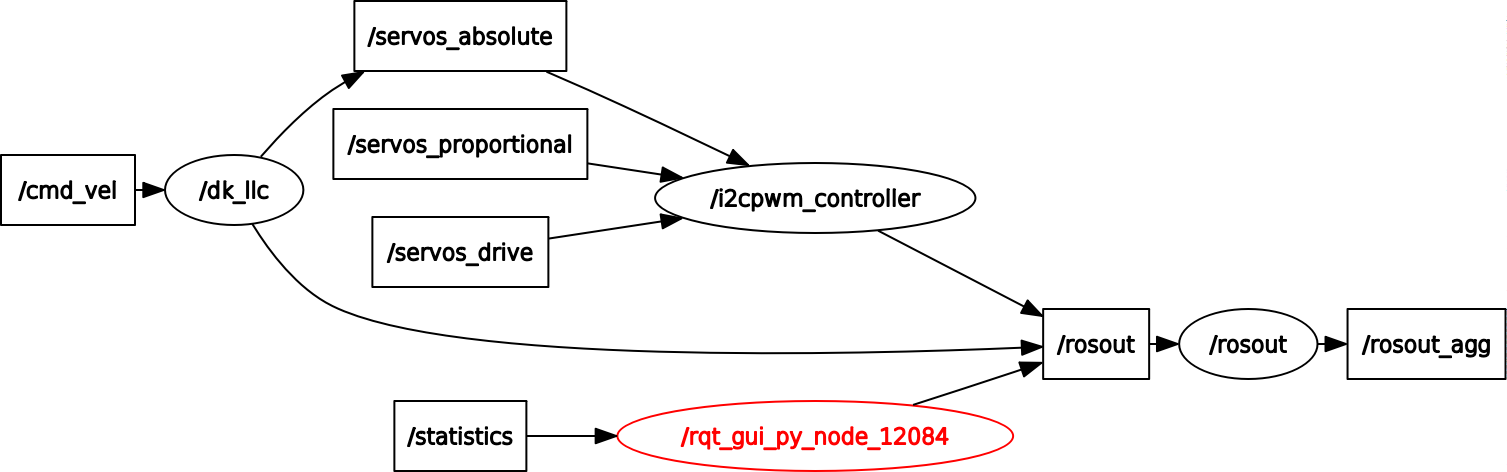
\includegraphics[width=9cm]{img/rosgraph.png}
		\caption{Übersicht der ROS Elemente}
		\label{rosgraph}
	\end{figure}
	
	Treu nach den Prinzipien von ROS besteht die Software aus vielen ROS Nodes, welche als Oval dargestellt werden. 
	Jeder Node erledigt kleine Aufgaben und kann als Subscriber und/oder Publisher fungieren.
	Die Kommunikation zwischen Subscriber und Publisher erfolgt durch ROS Messages (Nachrichten).
	Diese werden durch verschiedene Topics — werden als Rechteck dargestellt — kommuniziert.
	Die Topics kann man als Kanäle für Nachrichten betrachten.
	
	Folgende Nodes befinden sich im Softwaresystem:
	\begin{itemize}
		\item /rosout (Master)
		\item /teleop\_twist\_keyboard (Fernsteuerung)
		\item /donkey\_llc (Hardwarenahe Steuerung)
		\item /ic2pwm\_board\_node (Bibliothek und Node zum Ansprechen des I2C-Protokolls und deren Verbindung mit ROS)
		\item serial\_node.py (Publisher der Ultraschallsensordaten)
	\end{itemize}
	
	Die zuvor genannten Nodes sind durch Topics miteinander verbunden und tauschen untereinander Nachrichten aus.
	Folgende Topics befinden sich im Softwaresystem:
	\begin{itemize}
		\item /cmd\_vel (command velocity, die Beschleunigungssteuerung)
		\item /servos\_absolute (Steuerung des Servos mit absoluten Impulsstart- und Stoppwerten)
		\item /servos\_proportional (Motorsteuerung für Geschwindigkeitsteuerung des Servos in seinem Bewegungsbereich)
		\item /servos\_drive (Lenken, Umwandlung der Berechnungen von Linear- und Winkeldaten in Servoantriebsdaten)
		\item /rosout (Standard ROS Output)
		\item /rangeMsg\_topic (Datenübertragung der Ultraschallsensordaten)
	\end{itemize}
	
	%----------------------------------------------------------------
	% Je nach Formatierung wird dies verändert werden dürfen und der pagebreak entfernt
	\pagebreak
	\subsubsection{Launchreihenfolge}%heike
	
	Dieses Kapitel ist eine Einleitung zum Starten der ROS Nodes und den 
	hierbei zu beachtenden Punkten. Ohne Vorkonfiguration und Launchfiles ist 
	die Knotenaufrufreihenvolge langwierig. Manche Schritte müssen auf einem 
	Laptop durchgeführt werden, andere via SSH auf dem Raspberry Pi.So muss 
	Laptop erfahren das der ROScore (Master Node) bereits auf dem Raspberry 
	Pi läuft.
	
	% Weitere Knoten werden noch folgen
	% ToDo: Zeilenumbruch
	\begin{minted}[frame=lines, breaklines=true 
	fontsize=\footnotesize,]{Bash}
	# Network ubiquityrobot03B
	# connect via SSH
	ssh ubuntu@10.42.0.1
	# enter password
	
	# 1. Console - on Raspberry Pi
	# Login via SSH
	cd catkin_ws/Robotic_AI_student_project/
	# If bash.rc wasn't changed to source workspace
	source devel/setup.bash
	rosrun i2cpwm_board i2cpwm_board
	
	# 2. Console - on Raspberry Pi
	# Login via SSH
	cd catkin_ws/Robotic_AI_student_project/
	source devel/setup.bash
	rosrun donkey_car low_level_control.py
	
	# 3. Console - on Laptop 
	export ROS_MASTER_URI=http://ubiquityrobot.local:11311
	export ROS_IP=$(hostname -I)
	cd catkin_ws/Robotic_AI_student_project/
	source devel/setup.bash
	rosrun teleop_twist_keyboard teleop_twist_keyboard.py
	
	# 4. Console - on Raspberry Pi
	# Login via SSH
	rosrun rosserial_python serial_node.py /dev/ttyACM0
	
	# 5. Console - on Laptop
	export ROS_MASTER_URI=http://ubiquityrobot.local:11311
	export ROS_IP=$(hostname -I)
	rostopic echo rangeMsg_topic
	\end{minted}
	
	Mehrere Schritte sind Möglich um diesen Prozess zu vereinfachen. Die 
	meisten Optionen sind eine frage der persönlichen Präferenz des ROS 
	Benutzers.  So kann ein Eintrag in die Systemweit geltende Datei 
	\textit{bash.rc} die Eingabe von \textit{source devel/setup.bash} im ROS 
	workspace ersetzen. \\
	Eine weitere Erleichterung ist der Eintrag eines Shellscripts in die 
	setup.bash Datei. \ref{Einzeiler} Dieser Eintrag Setzt die ROS Host IP 
	Variable auf die aktuelle IP Adresse des Laptops.
	\begin{figure}
		\centering
		\begin{minted}[frame=lines,breaklines=true,
		fontsize=\footnotesize,
		framesep=2mm
		]{Bash}
		export ROS_IP=$(ip -br -4 address show dev wlp3s0 | awk '{print $3}' | 
		awk -F '/' '{print $1}')
		\end{minted}
		\label{Einzeiler}
		\caption{Bash Einzeiler, Autor J.K }
	\end{figure}
	\\
	Eine weitere Möglichkeit der Vereinfachung besteht im erstellen von 
	SSH-Keys. 
	
	\subsubsection{Launchfiles}
	
	Launchfiles die viele ROS Knoten auf einmal starten sind eine Beliebte 
	Vereinfachung. Um die \textit{Keyboard Demo}  \ref{demo} zu starten, oder 
	den Roboter Fernzusteuern existiert ein Lauchfile im \textit{Donkey Car} 
	Fork 
	des Github Quelle.
	\begin{figure}
		\centering
		\begin{minted}[frame=lines,breaklines=true,
		fontsize=\footnotesize,
		framesep=2mm
		]{Bash}
		#call on Raspbeery Pi to launch hardware nodes
		roslaunch donkey_car keyboard_demo.launch
		#call keyboard node from laptop 
		rosrun teleop_twist_keyboard teleop_twist_keyboard.py
		\end{minted}
		\label{demo}
		\caption{Tastatur Steuerung per Launchfile }
	\end{figure}
	
	Um die benötigten Knoten Für die Künstliche Intelligenz komfortabel zu 
	starten wurden zwei Launchfiles geschrieben \ref{KI-launch} .  Das ist 
	Notwendig da die 
	Anwendung verteilt läuft. (siehe spätere Artikel)
	
	\begin{figure}
		\centering
		\begin{minted}[frame=lines,breaklines=true,
		fontsize=\footnotesize,
		framesep=2mm
		]{Bash}
		#call from Raspberry Pi
		roslaunch donkey_car hardware.launch
		#call from Laptop
		export ROS_MASTER_URI=http://ubiquityrobot.local:11311
		roslaunch ki_nav start_AI.launch
		\end{minted}
		\label{KI-launch}
		\caption{Künstliche Intelligenz starten per Launchfile }
	\end{figure}
	%----------------------------------------------------------------
	
	\section{Praktische Projektdurchführung}
	
	%----------------------------------------------------------------
	
	In diesem Kapitel wird der Hardwareaufbau des rosBerry, sowie die mechanisches Bauteile inklusive Entscheidungskriterien vom Roboter beschrieben. 
	Hierfür werden die einzelnen verwendeten Hardwarekomponenten — deren Modell und Funktion — vorgestellt. 
	
	Zuerst werden die Verbindungen der Hardwarekomponenten untereinander abgebildet, wie in Abbildung \ref{Hardwarekomponenten} zu sehen.
	\subsection{Mechanische Bauteile}
	
	\begin{figure} %[!h]
		\centering
		%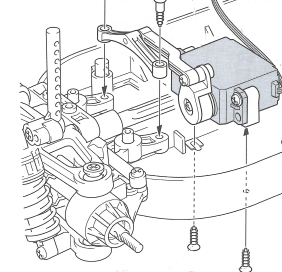
\includegraphics[width=9cm]{img/servo.png}
		\caption{Auszug aus Hersteller Datenblatt:Lenkservo }
		\label{Servomotor}
	\end{figure}
	Für das Robotik Projekt \textit{rosBerry} wurde ein solides, aber günstiges Chassis gesucht bei dem die Möglichkeit besteht Ersatzteile zu bestellen. Viele qualitativ hochwertige Modellbau Chassis liegen in einem Preisrahmen über 400€, für diese ist die Ersatzteilbeschaffung gut möglich. Günstige, meist asiatische Modellbau Chassis Hersteller liefern ihre Modelle und Bausätze nur für einen kurzen Zeitraum. Es ist oft nicht möglich zu einem späteren Zeitpunkt das Modell nachzukaufen oder Ersatzteile zu bekommen. Somit ist ein Roboter der darauf aufbaut, wie das Donkey Car, nicht reproduzierbar. 
	\\
	\begin{figure} %[t]
		\centering
		%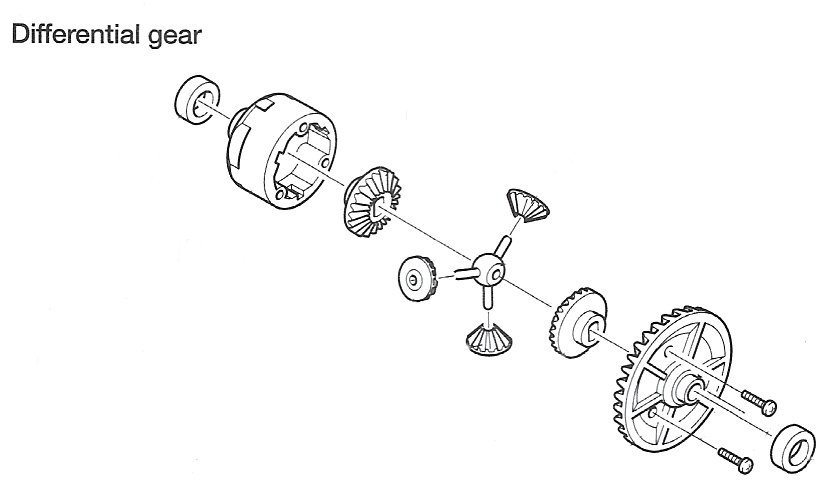
\includegraphics[width=9cm]{img/geer.png}
		\caption{Auszug aus Hersteller Datenblatt: Differnzialgetriebe }
		\label{Getriebe}
	\end{figure}
	Der Kompromiss dieser Abwägung fand sich bei einem älteren 
	Einsteigermodell namens TAMIYA RC 1:10 TT-01E. Tamiya ist ein 
	traditionsreicher japanischer Hersteller der qualitativ hochwertige Bausätze 
	ferngesteuerte Fahrzeuge herstellt. (Er stellt Schiffe, Flugzeuge und Panzer 
	her, aber hauptsächlich Modellautos) Tamiya ist unter 
	Modellbau-Enthusiasten dafür bekannt, alle Prinzipien japanischer 
	Ingenieurskunst bei der Konstruktion seiner Modelle anzuwenden, statt 
	\textit{Spielzeugqualität} in China herzustellen. Das TT01-Modell hat 
	identische Außenmaße und kann mit denselben elektronischen Komponenten 
	betrieben werden, wie sein Nachfolgemodell das TT02. Somit ist die 
	Reproduzierbarkeit im Bezug auf das Chassis gegeben.
	\\
	Die Mechanik des \textit{TAMIYA RC 1:10 TT-01E } Modells basiert auf 
	einem Motor und einer langen Antriebswelle, die drei Differenzialgetriebe 
	bewegt. \ref{Getriebe} Die Modelle werden als Vierradantrieb vermarktet. 
	Die Lenkung wird Getrennt vom Antrieb durch einen Kleinen Servo Motor 
	geregelt\ref{Servomotor}. Er bewegt die Spurstange nach rechts/links. Das 
	Chassis nutzt also eine Akkerman Lenkung, wie sie auch bei PKWs üblich ist.
	
	\subsection{Elektronische Bauteile und ihre Funktion}
	% SVG ?
	\begin{figure} %[t]
		\centering
		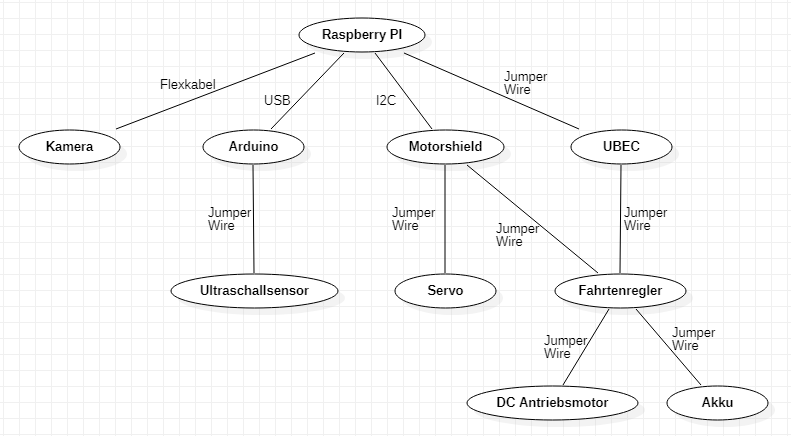
\includegraphics[width=9cm]{img/Hardwarekomponenten.PNG}
		\caption{Verbindungen der Hardwarekomponenten im rosBerry}
		\label{Hardwarekomponenten}
	\end{figure}
	
	Wie aus der Abbildung \ref{Hardwarekomponenten} zu erkennen, ist die meiste Hardware mit Jumper Wire verbunden.
	Ausnahmen der Anschlüsse bilden die Verbindungen des Raspberry Pis zur Kamera (Flexkabel), zum Arduino (USB) und zum Motorshield (I2C).
	\\
	
	Als Nächstes wird rosBerry mit den Hardwaremodellen vorgestellt.
	\\
	\begin{figure}[!ht]
		\centering
		\includegraphics[width=9cm]{img/RosBerryGesamt.png}
		\caption{Gerüst rosBerry}
		\label{rosBerryGesamt}
	\end{figure}
	
	Die verwendete Hardware ist in Abbildung \ref{rosBerryGesamt} mit Nummern versehen.
	Auf jede dieser Nummern wird referenziert und die Hardware mit Modell und Funktion aufgelistet.
	
	\begin{enumerate}
		\item Der DC-Antriebsmotor — Modell Tamiya Mabuchi RS 540 SH — steuert alle vier Räder des rosBerry an.
		Ohne ihn wird der Roboter nicht in Bewegung kommen.
		\item Neben dem DC Antriebsmotor befindet sich ein Fahrtenregler, Modell BORSTI 1/10 BRUSHED-ESC 45A.
		Dieser erhält vom Motorshield ein PWM-Signal, welches er verstärkt.
		Das verstärkte PWM-Signal wird anschließend in Geschwindigkeit umgesetzt und an den DC-Antriebsmotor weitergeleitet.
		\item Der UBEC — Modell HWBEC Hobbywing 3A \SI{5}{V} \SI{6}{V} max \SI{5}{A} — wird eingebaut, um den Raspberry Pi mit \SI{5}{V} zu versorgen.
		Ohne den UBEC würde der Raspberry Pi aufgrund der höheren elektrischen Spannung beschädigt werden.
		\item Der Servo — Modell Amewi AMX Racing 4806HB — bekommt vom Motorshield ein PWM Signal übermittelt.
		Nach dem PWM Signal richten sich die beiden Reifen aus und ermöglichen eine Fahrtrichtung.
		Dadurch ist rosBerry in der Lage links\,/\,rechts Kurven sowie geradeaus zu fahren.
		\item Der Akku dient dazu, die Stromversorgung des Roboters zu sichern.
		Dieser hat eine Nennspannung von \SI{7,2}{Volt}. Er versorgt die Hardware mit Strom.
		\item Der Motorshield — Modell Adafruit 16-Channel 12-bit PWM/Servo Driver-I2C interface PCA9685 — wird für die Geschwindigkeit und die Richtung der Reifen eingesetzt.
		Hierzu erzeugt der Motorshield zwei PWM Signale.
		Das 1. PWM Signal wird an den Servo übermittelt, um den Servo in die gewünschte Position einzustellen.
		Das 2. PWM Signal wird erzeugt und zum Fahrtenregler gesendet.
		Dieses wird zur Einstellung der Geschwindigkeit verwendet.
		\item Der Raspberry Pi 3.B+ ist das Herzstück des rosBerry.
		Auf ihn läuft zum einem ROS und zum anderen die Software des Roboters, welche im Kapitel ROS Knoten Software Architektur vorgestellt wurde.
		Über eine I2C-Schnittstelle werden Daten an den Motorshield übertragen.
		Die Daten geben an, wie das PWM Signal auszusehen hat.
		\item Der Arduino UNO REV 3 steuert einen Ultraschallsensor an und erzeugt einen ROS-Knoten (Publisher).
		Innerhalb des Programms wird das Signal des Sensors in Meter umgewandelt und in eine Range Message gespeichert.
		Die Range Message namens rangeMsg wird an das Topic rangeMsg\_topic übermittelt.
		Ein Subscriber — der auf dem Raspberry Pi läuft — subscribed das Topic und erhält regelmäßig Sensordaten über die Reichweite.
		
		\begin{figure}
			\centering
			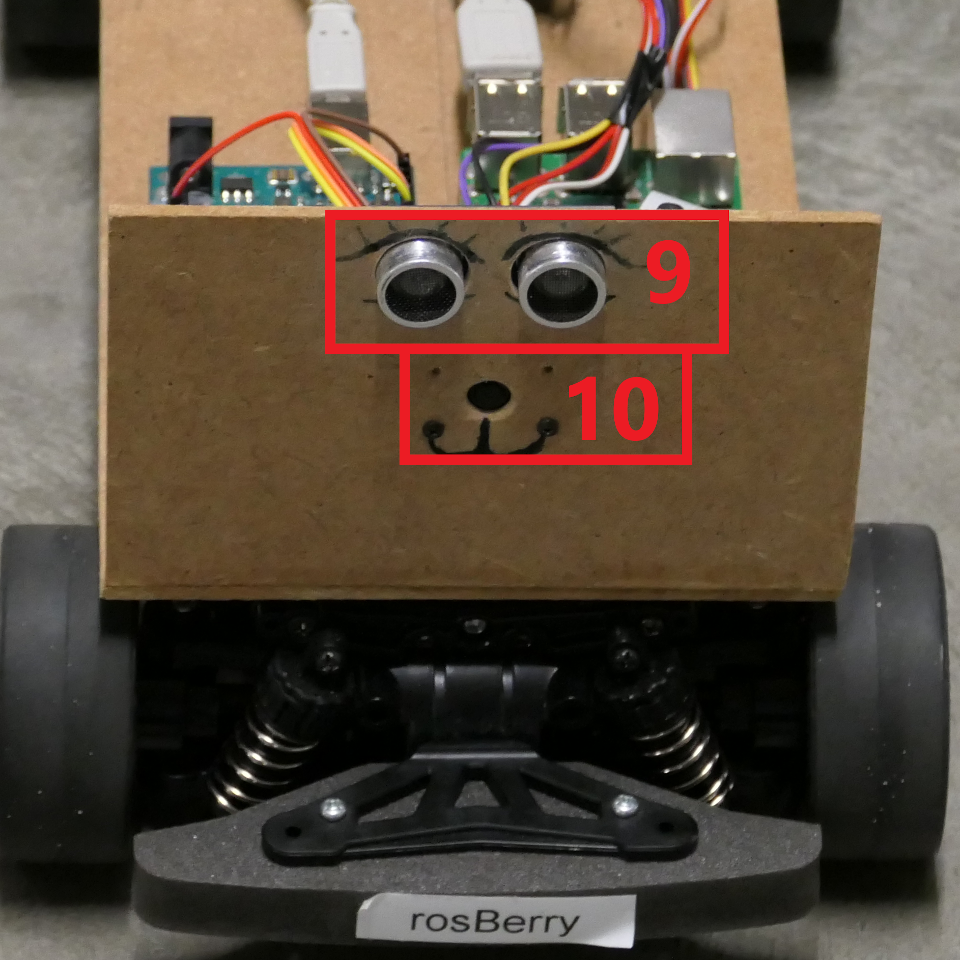
\includegraphics[width=5.5cm]{img/RosBerryWeitere.png}
			\caption{Weitere Hardwareelemente}
			\label{rosBerryWeitere}
		\end{figure}
		\item Der Ultraschallsensor — Modell HC-SR04 — wird zum rechtzeitigen Erkennen eines kommenden Hindernisses eingesetzt.
		Dieser hat eine maximale Reichweite von vier Meter, jedoch haben wir uns für das Projekt auf eine Reichweite von 2 Meter geeinigt.
		Alle 1/4 Sekunde sendet dieser ein Signal und verarbeitet dieses.
		\item Die Kamera — Modell 5 MP — ist durch ein Flexkabel an den Raspberry Pi über das CSI-Interface angeschlossen.
		Diese versorgt die KI mit Bildern, welche einen Marker sucht und findet.
	\end{enumerate}
	
	%----------------------------------------------------------------
	
	
	\section{Autonomes Verhalten durch Künstliche Intelligenz}	%mary
	
	Ziel des KI-Teils des Projektes besteht darin, dem Roboter beizubringen, einem optischen Marker zu folgen.
	Dazu muss er erst einmal das Symbol erkennen, dann herausfinden in welcher Richtung sich der Marker befindet.
	Danach erst kann er auf den Marker zufahren.
	\\
	
	Der schwierigste Teil der Aufgabe besteht darin, den Marker zuverlässig in unterschiedlichen Umgebungen zu erkennen.
	
	\subsection{Erster Ansatz für das Neuronale Netz}	%steffen ? mary?
	%netzaufbau am anfang
	Der erste Entwurf unseres Neuronalen Netzes war stark angelehnt an F. Grovers Beispielnetz aus \glqq Artificial Intelligence for Robotics\grqq \cite{govers2018artificial}. Wie in der Vorlage erstellen wir ein sequentielles Modell mithilfe von Keras.
	
	Die erste Schicht stellt ein convolution layer mit 20 convolutions dar, wovon jede ein Merkmal des Eingangsbildes isolieren soll.
	Die Größe setzen wir auf 5x5, betrachten also zwei benachbarte Pixel in jede Richtung.
	Selbstverständlich muss dafür auch ein Padding hinzugefügt werden, damit das Verfahren auch am Bildrand funktioniert. 
	
	Zudem wird noch eine Aktivierungsfunktion benötigt, hierfür nutzen wir die ReLU-Funktion, die nur positive Werte zulässt und negative Werte durch den Wert 0 ersetzt.
	Diese Aktivierungsfunktion ist deshalb sinnvoll, da das Ergebnis als Farbe dargestellt werden und deshalb einen Wert zwischen 0 und 1 annehmen soll.
	Ein Wert unter Null wäre hier unbrauchbar.
	
	\begin{minted}[frame=lines]{Python}
	model = Sequential()
	inputShape = (height, width, depth)
	
	model.add(Conv2D(20, (5, 5), padding="same", input_shape=inputShape))
	model.add(Activation("relu"))
	\end{minted}
	
	Die zweite Schicht ist ein Maxpooling-Layer, bei dem wir jeweils 2x2 Pixel nehmen und danach 2x2 Pixel weiterrücken um keine Überlappungen zu haben.
	Das Ergebnis ist ein Bild in ¼ der originalen Größe: aus 640x480px wird 320x240px, aus 128x128px 64x64px usw.
	
	Direkt darauf folgt ein weiteres convolution layer mit der doppelten Anzahl an convolutions — 40 statt vorher 20 — um mehr Mermale zu identifizieren.
	Durch das vorher durchgeführte maxpooling werden nun andere, größere Merkmale erkannt.
	Ebenfalls nutzen wir wieder dieselbe ReLU Aktivierungsfunktion, aus denselben Gründen wie in der ersten Schicht.
	
	\begin{minted}[frame=lines]{Python}
	model.add(MaxPooling2D(pool_size=(2, 2), strides=(2, 2)))
	model.add(Conv2D(40, (5, 5), padding="same"))
	model.add(Activation("relu"))
	\end{minted}
	
	%\begin{lstlisting}[label={list:model_1_2},caption=Modell: zweite und dritte Schicht]
	%	model.add(MaxPooling2D(pool_size=(2, 2), strides=(2, 2)))
	
	%	model.add(Conv2D(40, (5, 5), padding="same"))
	%	model.add(Activation("relu"))
	%\end{lstlisting}
	
	Schicht vier besteht erneut aus einem Maxpooling-Layer, ebenfalls um nochmals größere Merkmale zu erkennen.
	Aus einem 640x480px großen Bild wird nun 160x120px, aus 128x128px sogar nur noch 32x32px.
	
	Darauf folgt nun eine Schicht, die vorher noch nicht im Neuronalen Netz vorkam:
	Zuerst werden die dreidimensionalen Bildinformationen mit der Funktion Flatten() in ein eindimensionales Array geplättet, bevor wir eine vollverknüpfte Schicht mittels Dense(500) hinzufügen.
	Erneut nutzen wir die ReLU Aktivierungsfunktion, aus bekannten Gründen.
	
	\begin{lstlisting}[label={list:model_1_3},caption=Modell: vierte und fünfte Schicht]
	model.add(MaxPooling2D(pool_size=(2, 2), strides=(2, 2)))
	
	model.add(Flatten())
	model.add(Dense(500))
	model.add(Activation("relu"))
	\end{lstlisting}
	
	Abschließend benötigen wir zwei Neuronen für die beiden Ausgangswerte "Marker" und "kein Marker".
	Zur Aktivierung nutzen wir die Softmax-Funktion, die auch normalisierte Exponentialfunktion genannt wird.
	Sie transformiert mehrdimensionale Vektoren in einen Wertebereich zwischen 0 und 1, wobei alle Komponenten zusammen 1 ergeben müssen, das heißt wenn "Marker" einen Wert von 0,65 hat, muss "kein Marker" einen Wert von 0,35 haben. 
	Die Funktion kann durchaus für mehr als zwei Ausgangswerte genutzt werden, für unseren Anwendungsfall werden jedoch nicht mehr Ausgangswerte benötigt.
	
	\begin{lstlisting}[label={list:model_1_4},caption=Modell: finale sechste Schicht]
	model.add(Dense(2))
	model.add(Activation("softmax"))
	\end{lstlisting}
	
	\subsubsection{Erste Auswertung der Ergebnisse}	%steffen? 
	%wiso war das scheisse 
	%weil wir einfach das Beispiel aus dem Buch kopiert haben…
	//kommt noch
	\subsection{Schritte zur Verbesserung der Erkennungsrate} %mary
	%was haben wir dann gemacht 
	
	
	\begin{figure}[!h]
		\centering
		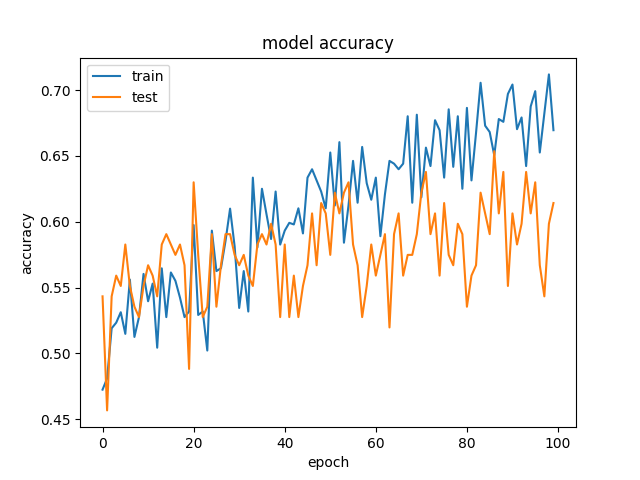
\includegraphics[width=9cm]{img/160x120:100@32_accuracy.png}
		\caption{erster Durchlauf}
		\label{Initiales Ergebnis}
	\end{figure}
	Beim ersten Durchlauf des Neuronalen Netzes war die Erkennungsrate des Markers 57\%. Dieses Ergebnis ist bei einer 50/50 Chance kaum besser als Raten.\\
	
	Die Schritte von  \glqq Learn Keras for Deep Neural Networkss\grqq \cite{moolayil2019learn} zum verbessern des Designs von Neurnalen Netzen wurden zur verbesserung der Trainignsergebnisse verwedet. 
	
	\cite{moolayil2019learn} Rät dazu mit einer kleinen Architektur anfangen das bedeutet wenige Schichten und wenige Neuronen. Es liegt nahe das kleine Architekturen Ressourcen schonender sind als grosse Architekturen. Dieser ansatz erscheint sinnvoll da Steigende Resourcenanforderngen bei gleichbleibender Hardware zu steigender Rechenzeit pro Epoche bedeuten. \\
	
	Das Netz nutzte anfangs nur eine Auflösung von 128x128 Pixel und 100 Epochen. Da jedes einzelne Pixel eine Eingangsneurone wird, ist anzunehmen, dass die geringe Auflösung im Buch gewählt wurde, um Rechenleistung zu sparen. \\
	
	\begin{figure}[!h]
		\centering
		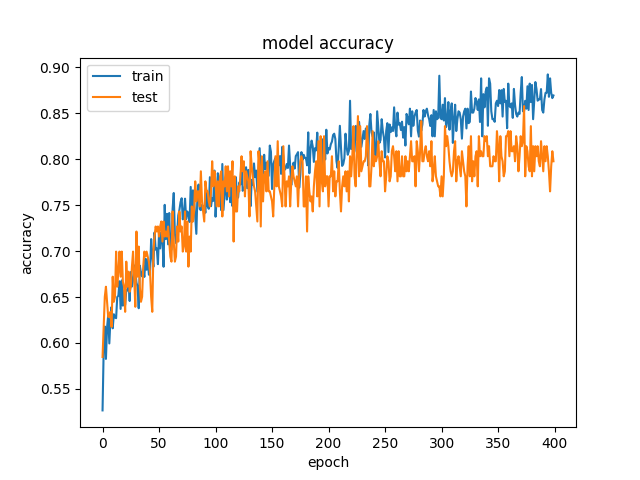
\includegraphics[width=9cm]{img/213x160:400@32_accuracy.png}
		\caption{overfitting}
		\label{Overfitt }
	\end{figure}
	
	\cite{moolayil2019learn} Rät die Anzahl an Neuronen pro Schicht erhöhen, wenn Anfangs kein befriedigenden Ergebnisse erzieht werden.
	Bei voller Bildauflösung von 640x480 Pixel erweist sich das Neuronale Netz auf der Hardware eines handelsüblichen Laptops als nicht mehr lauffähig. Für weitere Durchläufe wurden die nächsten Versuche auf einer Workstation mit mehr Grafkikkarten und Deutlich mehr RAM gemacht. Die Erkennungsrate stieg bei größerer Auflösung und mehr Durchläufen tatsächlich auf über 80\%. Damit vergrösserte sich jedoch das Modell (die Gewichte der KI) auf über ein Gigabyte. Ein so großes Modell kann nicht zeitnahe auf einem Raspberry Pie angewedet werden, da es nicht mehr in den RAM passt. Auch auf Standart Laptops ist zu erwarten das ein größeres Modell echt zeit Berechnungen erschwert. \\
	
	
	Um mit einer höhreren Auflösung trainiren zu können wurden die nächsten Trainingseinheiten auf einem performateren Server durchgeführt. Der zusätzliche Arbeitsspeicher und die Grafikarten bringen bei einer aktivierung der CUDA beschleunigung einen grossen Geschwikdikeitszuwachs . \\
	
	Ein weiteres Problem das zu Tage trat war das Overfitting. Das Modell entwickelte sich gut auf Trainingsdaten, schnitt jedoch deutlich schlechter bei Testdaten ab, mit denen es nicht trainiert hatte. Die Kurven liefen bei mehr als 200 Epochen weit auseinander.\\
	
	
	Weiterhin Rät \cite{moolayil2019learn} mehr Schichten benutzen, Beispielsweise abwechselnd eine Dichte schicht( dense layer) und eine Dropout Schicht.
	
	Dropout Schichten im Neuronalen Netz verbesserten das Overfitting Problem. Somit waren mehr Trainingsläufe ohne overfitting möglich. Das neuronale Netz erreichte so werte von rund 85\%. \\
	
	Das Modell das TensorFlow bei voller Auflösung oder 307200 Eingangsneuronen erstellt ist über ein Gigabyte groß. Je größer das Modell ist, des do unwahrscheinlicher das ein Raspberry Pi das Modell in absehbarer Zeit auf ein Bild anwenden kann. Somit erwies sich der Ansatz einfach die Auflösung zu erhöhen als nicht  zielführend für den Anwendungsfall. \\
	
	Das Modell musste also kleiner werden ohne wesentliches Overfitting. Diese Ziehl wurde durch die Kombination von Dropoutschichten, mehr Durchläufen und kleinerer Pixelanzahl erreicht. \\
	
	\cite{moolayil2019learn} Rät weiterhin, die Daten neu analysieren, wenn eine weitere Steigerung der Anzahl an Schichten und der Neuronen keine weitere Steigerung der Erkennungsrate bringt. Es wurden als Bilder mit sehr geringem Kontrast aussortiert, extrem Dunkle Bilder sowie Bilder auf denen der Marker sehr weit entfernt war. Sie wurden durch Bessere Daten ersetzt. (neue Bilder wurden angefertigt jeweils mit und Ohne Marker) Dieser Schritt verursachte eine Merkliche Verbesserung des Trainingsergebnis.
	\\
	
	
	\begin{figure}[!h]
		\centering
		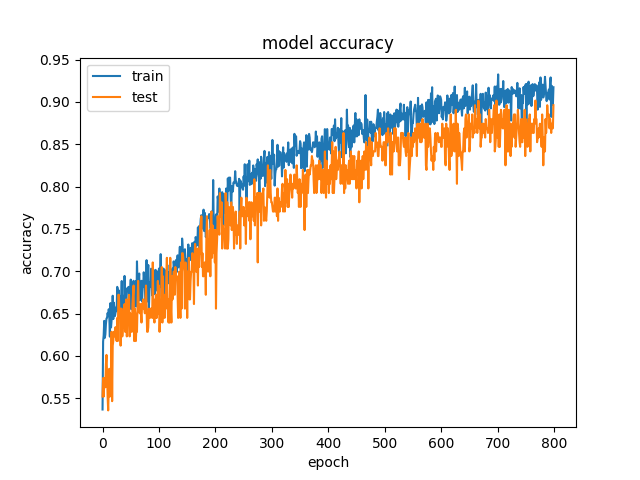
\includegraphics[width=9cm]{img/213x160:800@32:0_accuracy.png}
		\caption{End ergebnis}
		\label{end Ergenisse }
	\end{figure}
	
	Alle weiteren versucht das Model weiter zu verfeinern scheiterten. Die Ursache dafür ist nicht eindeutig geklärt. Eine mögliche Erklärung ist  das der Datensatz für die komplexität des Models zu klein war . Auch möglich ist das die Grenzen der Optimierer ADAM und Stochastic Gradient Descent erreicht waren. Auch Programmierfehler konnten nicht ausgeschlossen werden. 
	
	\begin{figure}[!h]
		\centering
		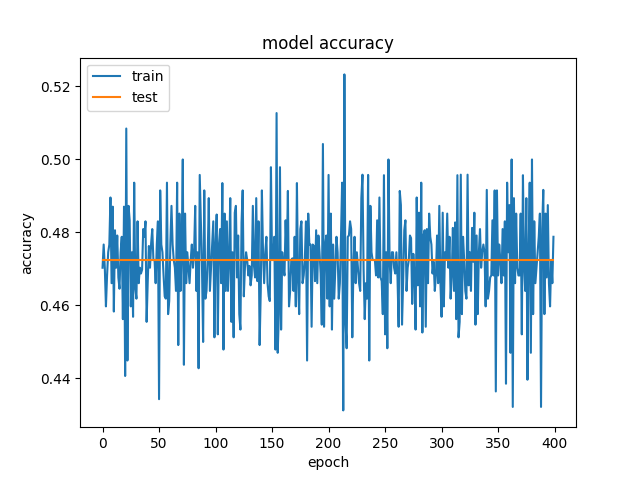
\includegraphics[width=9cm]{img/480x360:400@32_accuracy.png}
		\caption{Kein sichtbarer Trainingserfolg}
		\label{erfolgloos }
	\end{figure}
	
	
	\subsection{Anwendung des Trainingsmodells} %steffen
	//kommt noch
	\subsubsection{Keras und Tensorflow auf Raspberry Pie Hardware}
	Der initiale Plan sah vor, dass das neuronale Netz auf dem Raspberry Pi auszuwerten, damit der Roboter komplett autonom (ohne WLAN und externen Computer) fahren kann. Die Prozessorleistung und der RAM eines Raspberry Pies 3B+ ist zwar deutlich geringer als der eines Standard Laptops, aber die Nachteile eines verteilten Systems erschienen anfangs größer. So wirkte der architektonische Aufwand für  verteilte Systeme und  das Einarbeiten in die Bibliothek CV Bridge zum Versenden von Bildern mit ROS aufwendig. \\
	Die meisten gängigen Bibliotheken und Frameworks sind unabhängig vom Zielbetriebssystem auf 64Bit Wortbreite ausgelegt, so auch Tensorflow und Keras.  Das verwendete Ubuntu Image mit ROS für Raspberry Pi jedoch ist ein 32 Bit System. Das bedeutet, es gibt keine vorkompilierten Versionen von Tensorflow für das bisherige Setup. Das Kompelieren großer Tarfiles auf einem Raspberry Pi, dauert oft mehr als eine Stunde. Teilweise läuft der Raspberry Pi dabei so heiß, dass er abstürzt. Ein Ventilator erwies sich als hilfreich, um  Abstürze während des Kompilierungsprozesses zu verhindern. Tensorflow ist eine große Bibliothek deren Kompilierung aufwendig ist. 
	%https://qengineering.eu/install-tensorflow-2.2.0-on-raspberry-pi-4.html
	Sagt über den Raspberry Pi 4   : \\
	\say{The whole TensorFlow installation procedure from start to end takes many hours (±33 for Python, ±10 for the C++ library). } \\
	Es ist  anzunehmen, dass der Zeitaufwand für eine Kompilierung auf dem weniger Performanten Raspberry 3B länger dauert. Vor dem Hintergrund, dass es keine Garantie gibt, dass 64 Bit Libaries auf auf 32 Bit Systemen reibungslos funktionieren, ist eine Kompilierzeit von über einem Tag nicht akzeptabel. \\
	
	Die Entscheidung für ein verteiltes System wurde getroffen. Dabei zeigten sich weitere erwähnenswerte Inkompatibilitäten. Für jede ROS Version (Distribution) existieren vor gepackte Installationspakete für ein Ubuntu Betriebssystem. Nur mit diesem System sind sie komplett kompatibel. Das Betriebssystem Ubuntu 18.04 ist mit ROS Melodic vorgesehen. Während das Betriebssystem Python 2.7 und Python 3.6.9. nutzt ist ROS Melodic auf Python 2.7 angewiesen. Die Python Versionen sind inkompatibel. Tensorflow2 benötigt eine aktuelle Python Version, die von ROS Melodic nicht ohne weiteres unterstützt wird. \\
	
	Tensorflow1 ist zwar mit Python2.7 kompatibel, es ist jedoch nicht 
	Threadsave. Das erschien anfangs kein Problem, da keine parallele 
	Programmierung geplant war. Ein Prototyp-Programm mit Anwendung von 
	neuronalem Netz lief problemlos auf Mac mit Python3. Dieses Programm 
	sollte als Vorlage für einen ROS Knoten dienen. Auf Ubuntu in ROS traten 
	jedoch viele kryptische Fehlermeldungen auf.  Die Tatsache das Die 
	Fehlermeldungen bei gleicher Eingabe so unterschiedlich waren verwirrte 
	anfangs. \ref{ Error1}, \ref{Error2}, \ref{Error3}
	
	\begin{figure}
		\centering
		\begin{minted}[frame=lines,
		fontsize=\footnotesize,
		framesep=2mm]{Bash}
		Not found: Container localhost does not exist. 
		(Could not find resource: localhost/conv2d_2/kernel)
		[[{{node conv2d_2/Conv2D/ReadVariableOp}}]]
		\end{minted}
		\label{Error1}
		\caption{Localost existiert nicht}
	\end{figure}
	
	\begin{figure}
		\centering
		\begin{minted}[frame=lines,
		fontsize=\footnotesize,
		framesep=2mm]{Bash}
		InvalidArgumentError: Tensor 
		dropout__input:0, specified in either 
		feed_devices or fetch_devices
		was not found in the Graph
		\end{minted}
		\label{Error2}
		\caption{Unverständliche Fehlermeldung}
	\end{figure}
	
	
	
	\begin{figure}
		\centering
		\begin{minted}[frame=lines,
		fontsize=\footnotesize,
		framesep=2mm]{Bash}
		
		ValueError: Tensor Tensor
		("activation_5/Softmax:0",
		shape=(?, 2), dtype=float32) 
		is not an element of this graph.
		\end{minted}
		\label{Error3}
		\caption{Tensorflow Graphenelement unbekannt}
	\end{figure}
	
	Es stellte sich heraus das entweder ROS, Python, Tensorflow oder die Kernel 
	des Betriebssystems den Bildanalyse-Algorithmus als hochgradig 
	parallelisierbar erkannt hat. Der Algorithmus im  ROS Knoten nutzte mehr 
	als einen Thread bei der Ausführung um die Mehrkern CPU auszunutzen. 
	Die abschließende Uhrsache konnte zum zeit des Papers nicht geklärt 
	werden.
	Laut Victor Meunier's Blog[Referenz hier] %link 
	muss sichergestellt werden, dass jeder Thread seinen eigenen Graph und seinen eigene Session hat. Das Schlüsselwort \say{With} hilft den Kontext zu definieren. \ref{with} \\
	
	\begin{figure}
		\centering
		\begin{minted}[frame=lines,
		fontsize=\footnotesize,
		framesep=2mm]{python}
		with graph.as_default():
		with thread_session.as_default():
		\end{minted}
		\label{with}
		\caption{Verwendung von Initialisiertem Graph}
	\end{figure}
	
	
	Erst innerhalb dieses Blockes kann sicher auf das vortrainierte Modell zugegriffen werden, um damit eine Vorhersage zu machen.
	\subsubsection{Algorithmus zur Bildanalyse }
	\noindent \\
	// kommt noch 
	%mach ich! ~steffen 
	%echt? wann? ~marie
	%bild teilen
	%bild analysieren
	\subsection {Auswertung des Verhalten des Roboters}	% mary? %steffen? %heike?
	//kommt noch
	%macht er irgendwas sinnvolles? ist er klüger als eine eintagsfliege
	
	%der gute rosBerry hat zu viele false positives, ändert ab und zu die richtung
	%reagiert relativ langsam
	
	\section{Erkenntnisse }
	Auch wenn dieses Projekt sehr lehrreich für alle Beteiligten war, kann ein studentisches Semesterprojekt nicht an die Leistungen im Rahmen von echten Forschungsarbeiten, durchgeführt von Wissenschaftlern mit Master oder Doktor Titel, heranreichen. Nicht nur das Budget sondern auch das Fachwissen, sowie die zeitlichen Gegebenheiten unterscheiden sich stark. Dieses Kapitel wird zuerst darauf auf mögliche Verbesserungen für eventuelle Nachfolgeprojekte eingehen, um dann einige Erkenntnisse zusammenzufassen. 
	
	\subsection{Empfehlungen für nachfolge Projekte}
	
	Empfehlungen auf Basis der Erfahrungen mit diesem Projekt sind, zunächst die Verbesserungsvorschläge für die Roboter Hardware und Software, danach Ansätze für die KI.\\
	Da dieses Projekt immer wieder Probleme mit der Inkompatibilität der veralteten Python Version und aktuellen Bibliotheken hatte, wird ein Hardware und Software Stack empfohlen, der durchgehend das aktuelle Python 3 verwendet. Auch die Leistungsgrenzen des Raspberry Pi waren schnell erreicht. \\
	
	Empfehlungen:
	\begin{itemize}
		\item  Besser ein Raspberry Pi 4* als ein Raspberry Pi 3
		\item  SD Karte mit mehr als 32GB
		\item Betriebssystem Ubuntu 20* in 64 Bit Variante
		\item  ROS Neotic* auf allen Rechnern
	\end{itemize}
	*oder aktueller wenn verfügbar
	\subsection{Ansätze zur Verbesserung der Erkennung der Marker durch die K.I}
	
	Es ist zu überprüfen, ob ein Ecken erkennender Featurematchingalgorithmus nicht dem verwendeten Kantenerkennungsalgorithmus überlegen ist. Ansätze der künstlichen Intelligenz, die sich darauf konzentrieren \textit{wo} die gesuchten Merkmalspunkte  im Gesichtsfeld des Roboters ist, statt sich darauf zu beschränken \textit{ob} ein Merkmalspunkt detektiert wurde, versprechen eine präzisere Navigation. \\
	Es ist in Zukunft zu überprüfen, ob ein Training mit schwarzweiß Bildern einen ähnlichen Trainingserfolg bringt. Bei gleicher Auflösung brauchen RGB Bilder drei mal so viele Daten wie schwarzweiß Bilder, da sie drei mal so viele Farbkanäle brauchen. Das Umrechnen von Farbbildern in schwarzweiß Bilder ist dank Opencv keine rechenintensive Operation. Inwieweit zusätzliche Rechenoperationen die Serialisierungszeit , die Versandzeit und die Reserialisierung der Daten aufhebt sprengte den Rahmen dieser Arbeit. Inwiefern die Reduktion der Datenmenge das Gesamtsystem performanter macht ist noch zu überprüfen.
	\\
	Des Weiteren ist darauf hinzuweisen, dass es schon viele gute Algorithmen zur Navigation mit Hilfe von optischen Markern gibt, deren Evaluation jedoch den zeitlichen Rahmen dieses Projektes gesprengt hätten. Für zukünftige Projekte ist ein Vergleich der bereits existierender Lösungen empfehlenswert.
	
	% pageref gibt Zahl, nameref der Name der Section, ref ergibt II-C (Kapitel 2 Unterabschnitt C)
	% Referenz geht? \ref{sec:Architektur}
	
	\subsection{Fazit}
	//kommt noch
	\begin{comment}	%  how-to formeln 
	\begin{equation}
	a+b=\gamma\label{eq}
	\end{equation}
	\end{comment}
	\begin{comment}
	\paragraph{Positioning Figures and Tables} 
	Use the abbreviation 
	``Fig.~\ref{fig}'', even at the beginning of a sentence.
	
	\begin{table}[htbp]
	\caption{Table Type Styles}
	\begin{center}
	\begin{tabular}{|c|c|c|c|}
	\hline
	\textbf{Table}&\multicolumn{3}{|c|}{\textbf{Table Column Head}} \\
	\cline{2-4} 
	\textbf{Head} & \textbf{\textit{Table column subhead}}& \textbf{\textit{Subhead}}& \textbf{\textit{Subhead}} \\
	\hline
	copy& More table copy$^{\mathrm{a}}$& &  \\
	\hline
	\multicolumn{4}{l}{$^{\mathrm{a}}$Sample of a Table footnote.}
	\end{tabular}
	\label{tab1}
	\end{center}
	\end{table}
	
	\begin{figure}[htbp]
	\centerline{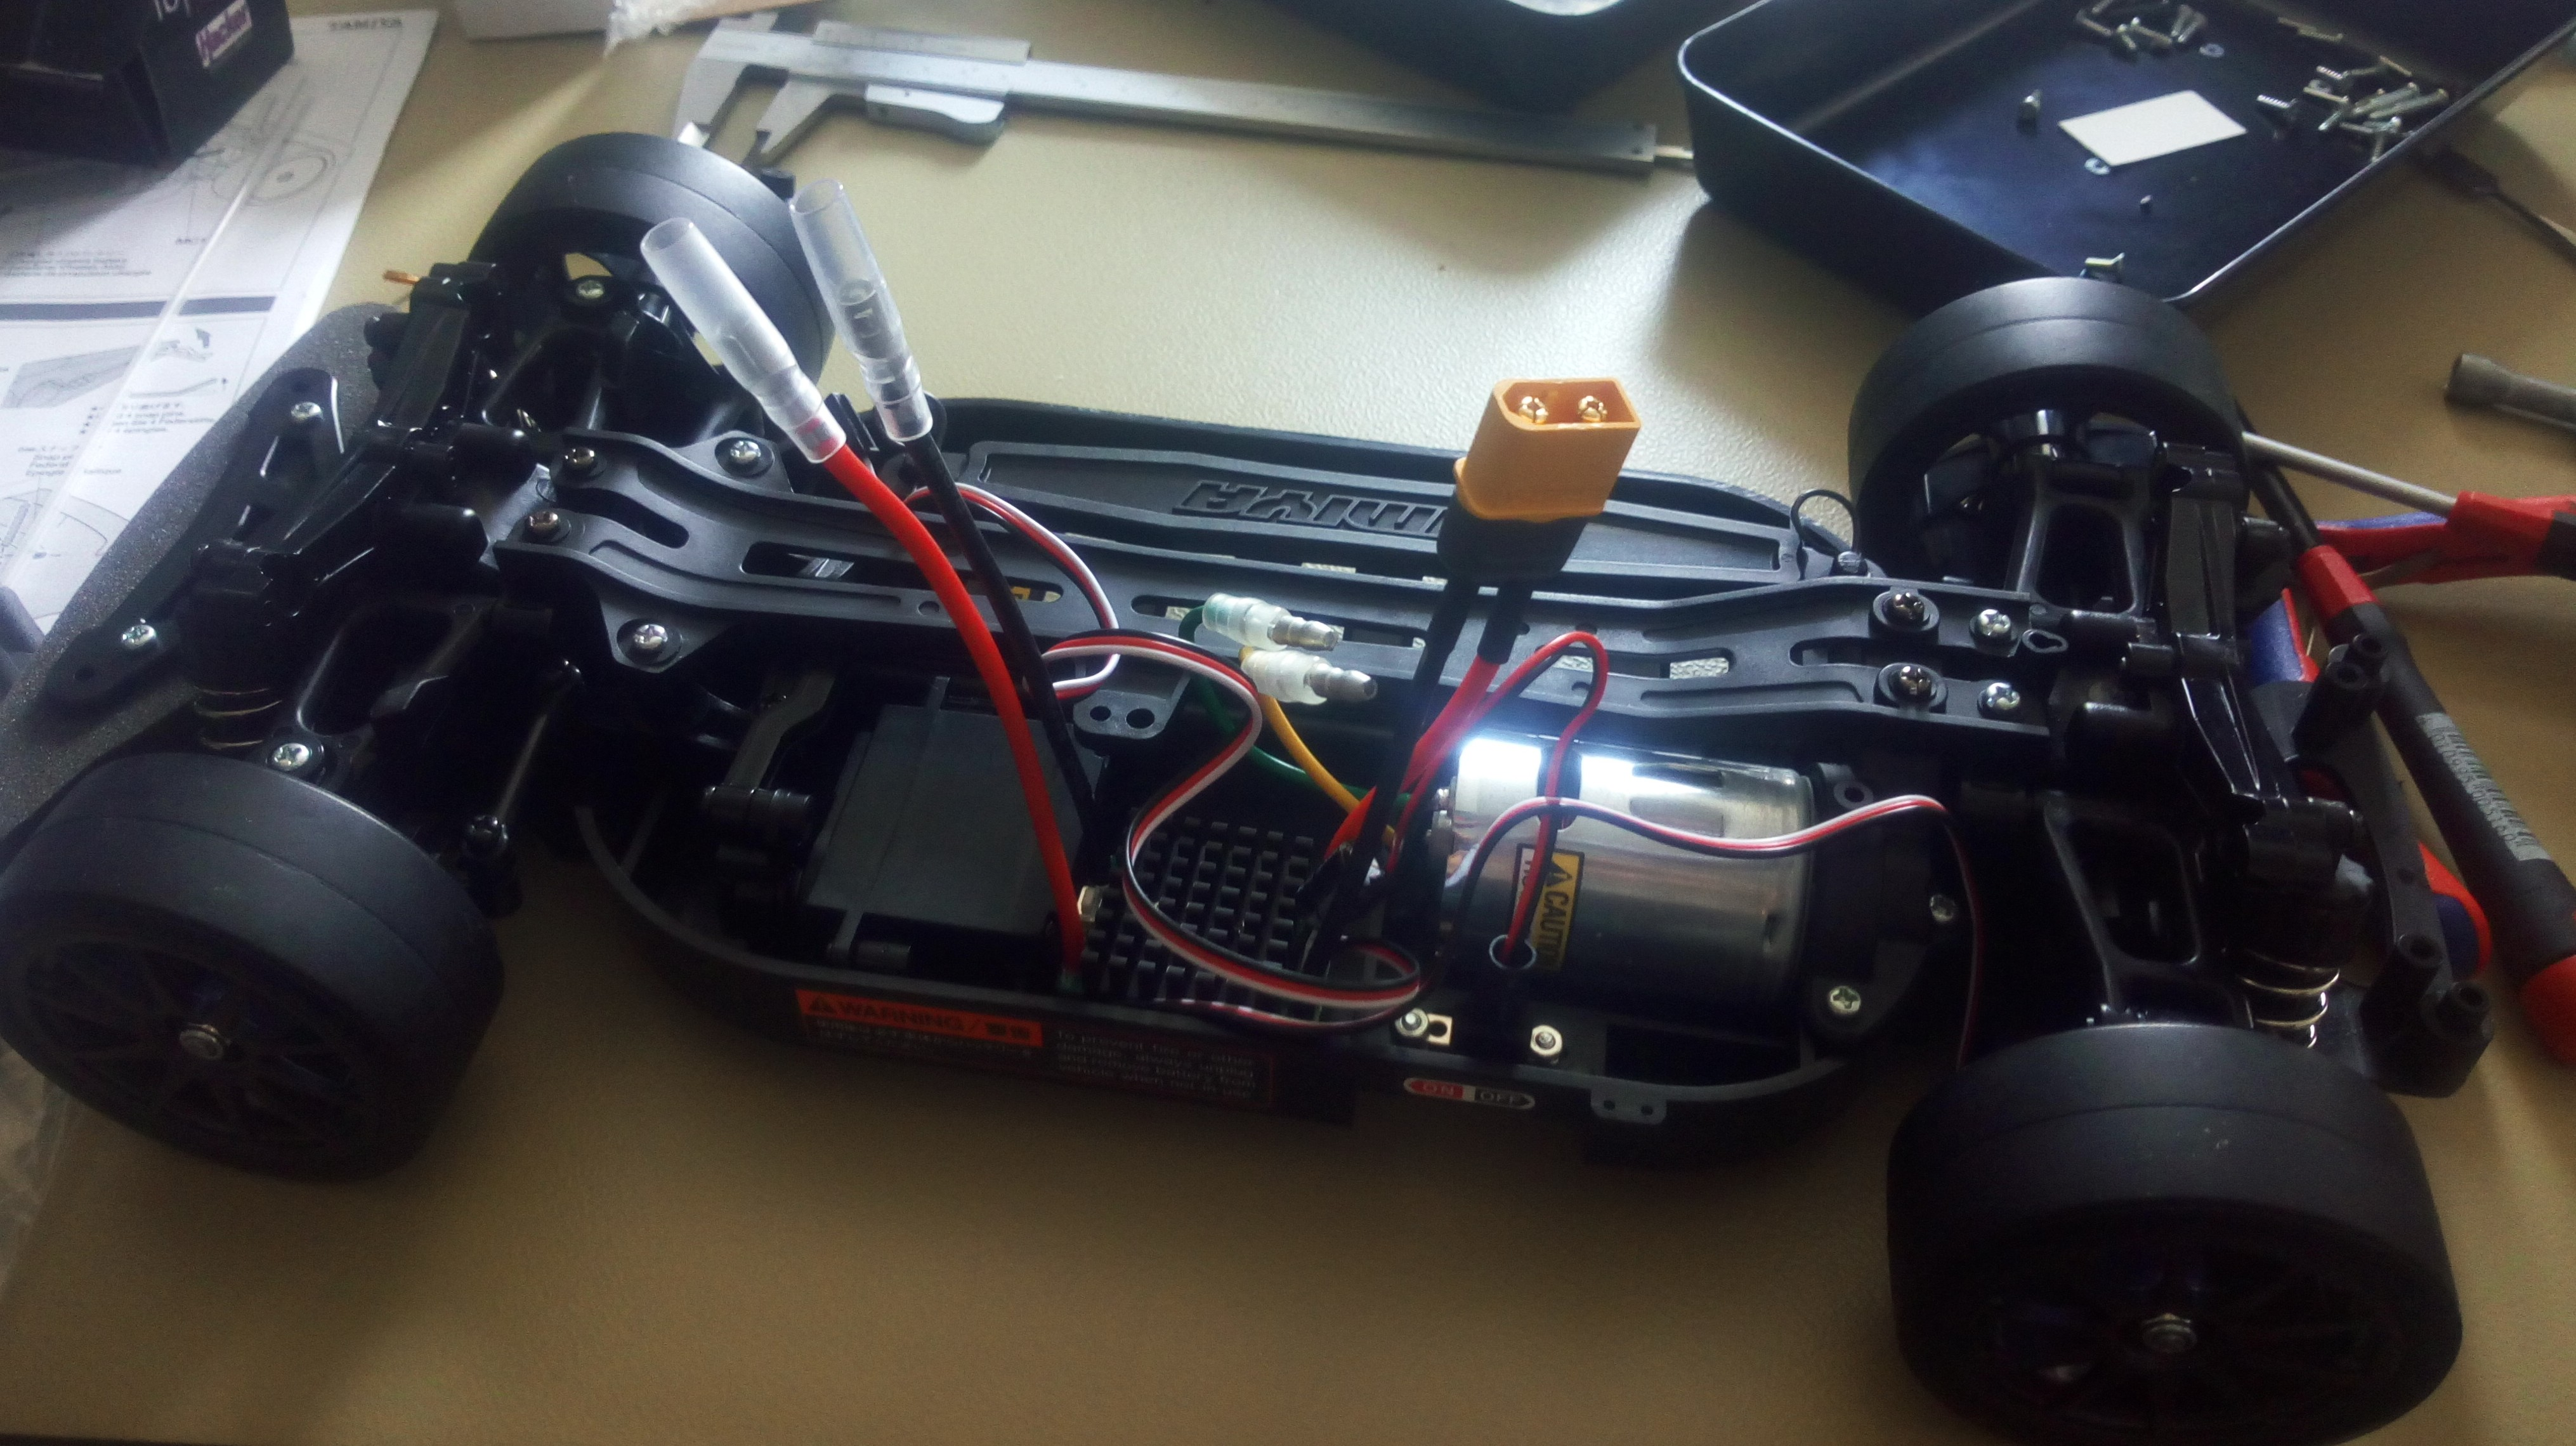
\includegraphics{img/car_body.jpg}}
	\caption{Example of a figure caption.}
	\label{fig}
	\end{figure}
	\end{comment}
	
	
	%\section*{Acknowledgment}
	% wollen wir unseren profs danken, weil mehr GPU und RAM? 
	
	% wissenschaftliche zitate gehen so \cite{b1}. 
	
	\begin{thebibliography}{00}
		\bibitem{b1}Francis X. Govers , Artificial Intelligence for Robotics, Packt Publishing ,2018
		\bibitem{b2}Amanda Decker , Bachelor Arbeit, Hochschule Mannheim ,2019	%keine wissenschaft
		\bibitem{b3}Learn Keras for Deep Neural Networks, Jojo Moolayil apress, 2019
		
		\bibitem{b4}https://www.tamiya.com/english/rc/manuals.htm	%keine wissenschaft
		\bibitem{b5}https://blog.victormeunier.com/posts/keras\_multithread/	%keine wissenschaft
		%TODO
		\begin{comment}
		%Bib file  neu machmen mit filter für wissenschaftliches und nicht wissenschaftliches
		%
		\defbibfilter{literatur}{%
		not type=url and not type=misc
		}
		
		\defbibfilter{web}{%
		type=url or type=misc
		}
		
		\printbibliography[filter=literatur,title={Literatur}]
		\printbibliography[filter=web,title={Web-Dokumente}]
		
		\end{comment}
		
	\end{thebibliography}
	
	% Dummy Cites zum Testen
	\cite{Amanda}
	\cite{Keras}
	\cite{Tamiya}
	\cite{govers2018artificial}
	\cite{moolayil2019learn}
	
	\printbibheading
	\printbibliography[filter=wissenschaftlich, heading=subbibliography, title={Fachliteratur}]
	\printbibliography[filter=nichtWissenschaftlich, heading=subbibliography, title={Web-Dokumente}]
	
\end{document}
